\documentclass[a4paper,11pt]{scrartcl}

\usepackage[utf8]{inputenc}
\usepackage[ngerman]{babel}
\usepackage[T1]{fontenc}
\usepackage{amsmath}
\usepackage{graphicx}
\usepackage{tabularx}
\usepackage[a4paper, left=2cm, right=2cm, top=2.8cm, bottom=2.8cm]{geometry}
\usepackage{tikz}   
%\usetikzlibrary{calc}

%defaultfam

%\usepackage[light]{montserrat}
%\usepackage{libertine}
\usepackage[scaled]{helvet}
%\usepackage[scaled]{uarial}

\renewcommand*{\familydefault}{\sfdefault}

\usepackage{tabto} 

\usepackage{fancyhdr}
\pagestyle{fancy}
\lhead{Maximilian Hoffmann}
\chead{Betrieblicher Auftrag \\ \textbf{Kabeltester}}
\rhead{
\includegraphics[width=3cm]{Bilder/BMK_LOGO.png}}

\begin{document}

\begin{center}
	\begin{huge}
	\textcolor{white}{\tiny{Platzhalter wenn ein Kapitel auf einer neuen Seite beginnt\\}}
	\textbf{Bedienungsanleitung}
	\end{huge}
\end{center}

\section{Bedienung}

\begin{center}
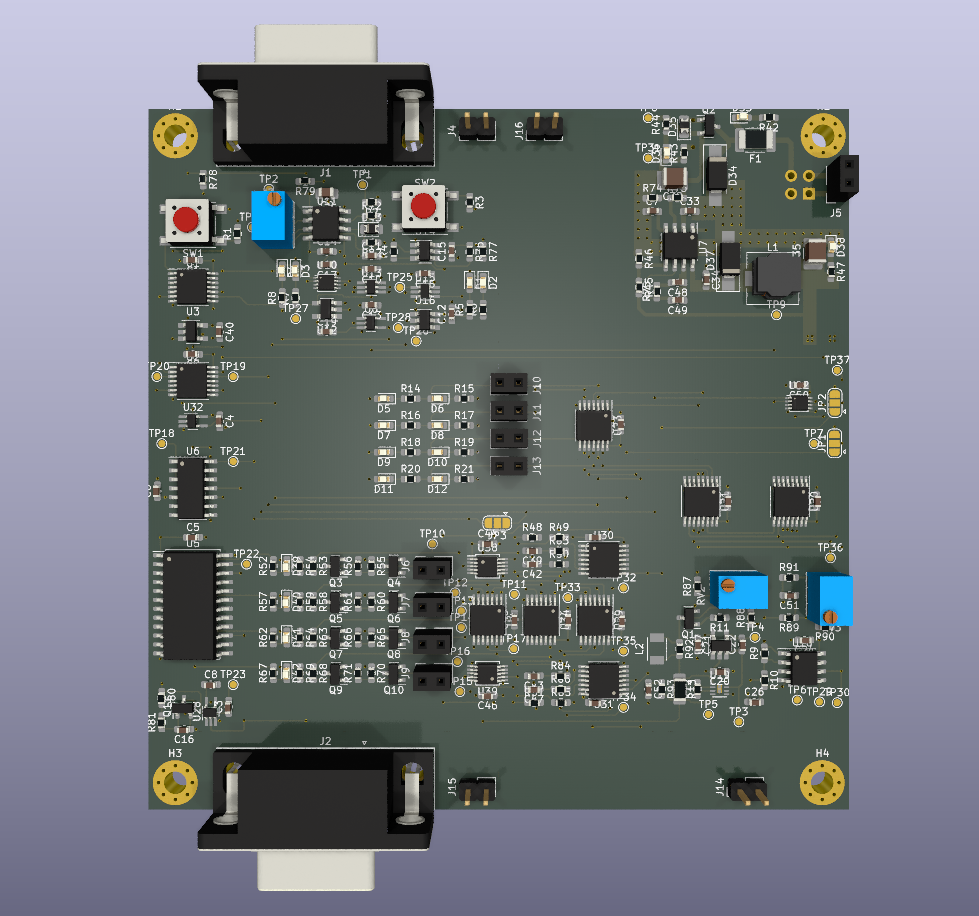
\includegraphics[width=15cm]{Bilder/Kabeltester-superbild.png}
\end{center}

\begin{itemize}
	\item[1] Umschalten zwischen \glqq Master\grqq und \glqq Slave\grqq Modus.\\
				\textbf{Mastermode:} Grüne LED leuchtet. Platine verwendet ihren internen Takt.\\
				\textbf{Slavemode:} Rote LED leuchtet. Platine verwendet externen Takt.
				
	\item[2] Messgeschwindigkeit kann geringfügig geändert werden.
	
	\item[3] Messung kann gestartet werden.
	
	\item[4] Messstrom und Grenzwiderstand können eingestellt werden.\\
	 			!Achtung! nach jeder Änderung muss der Teil neu kalibriert werden.
	 			
	\item[5] Zwischen diesen beiden Anschlüssen muss das zu messende Kabel gesteckt werden.
	
	\item[6] Jumper stecken.
	
	\item[7] Optische Ausgabe / Feedback.
\end{itemize}

\newpage

\section{Programmierkabel-Test}

Um ein Programmierkabel testen zu können muss ein passender Adapter gefertigt werden. Da die Schaltung Kurzschlüsse nur bei parallel verlaufenden Adern detektieren kann, müssen Kreuzungen der Adern durch eine zusätzliche Adapterplatine entfernt werden. 
\\
\\
Dies könnte so aussehen:

\vspace{1cm}

\begin{center}
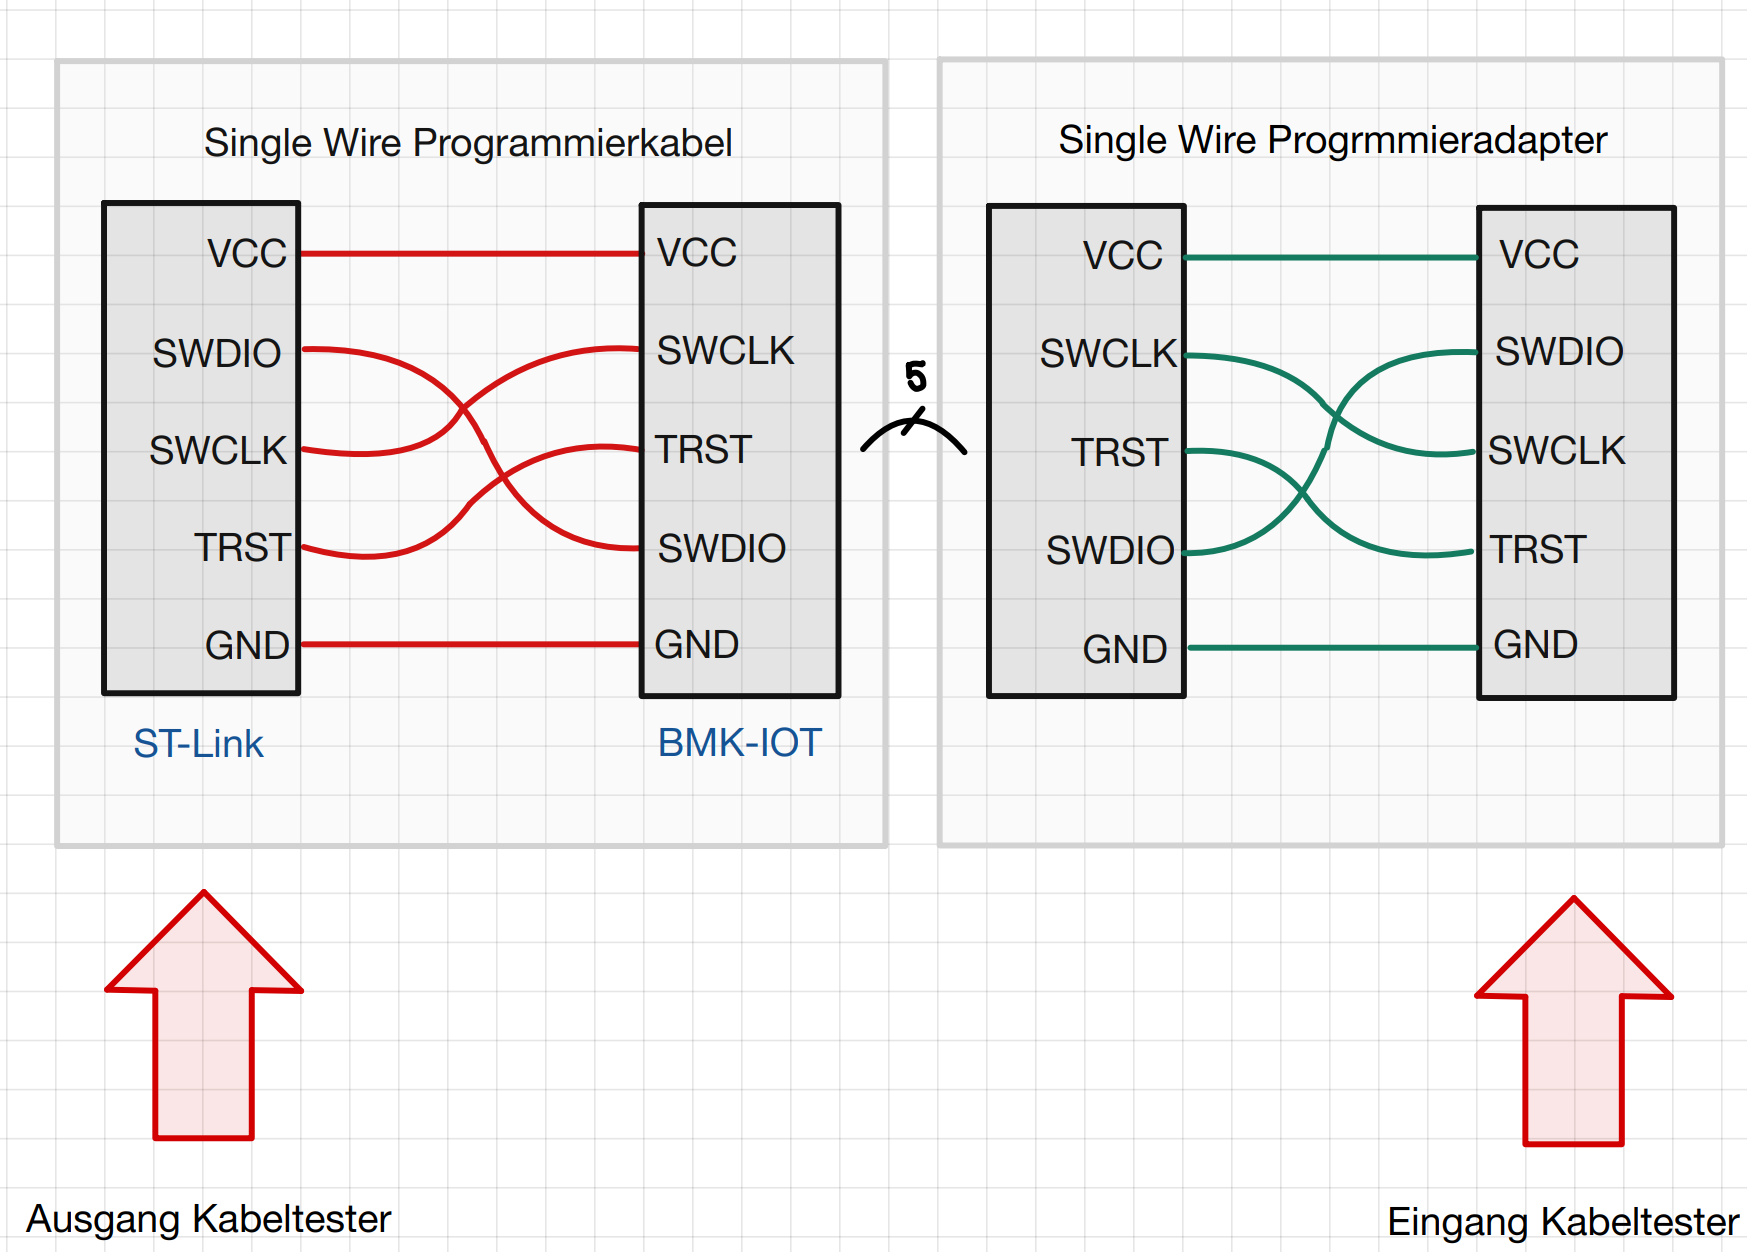
\includegraphics[width=15cm]{Bilder/Adapter.png}
\end{center}

\end{document}
